\documentclass[tikz,border=10pt]{standalone}
\usetikzlibrary{positioning}
\tikzset{main node/.style={rectangle,draw,minimum size=14pt,inner sep=2pt}}
\tikzset{outlierStyle node/.style={rectangle,minimum size=1cm,inner sep=0pt}}
\begin{document}
  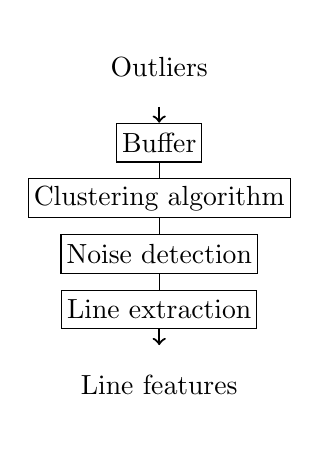
\begin{tikzpicture}
    \node[outlierStyle  node] (1) {Outliers};
    \node[main node] (2) [below = 0.2cm of 1]{Buffer};
    \node[main node] (3) [below = 0.2cm of 2]{Clustering algorithm};
    \node[main node] (4) [below = 0.2cm of 3]{Noise detection};
    \node[main node] (5) [below = 0.2cm of 4]{Line extraction};
    \node[outlierStyle node] (6) [below = 0.2cm of 5]{Line features};

    \draw[thick,->] (1) -- (2);
    \draw (2) -- (3) -- (4) -- (5);
    \draw[thick,->] (5) -- (6);
\end{tikzpicture}
\end{document}